% !Mode:: "TeX:UTF-8"
% !TEX program  = xelatex
\documentclass[a4paper]{article}
\usepackage{amsmath}
\usepackage{amssymb}
\usepackage{enumerate}
\usepackage{amstext}
\usepackage{ctex}
%\usepackage{braket}
\usepackage[european]{circuitikz}
\usepackage{multirow}
\usepackage{graphicx}
\usepackage{subfig}
\usepackage{float}
\usepackage{url}
%\usepackage[table,xcdraw]{xcolor}
\usepackage{colortbl}
\usepackage{geometry}
\geometry{left=2.5cm,right=2.5cm,bottom=2.5cm,top=2.5cm}

\title{模电实验报告8:波形发生电路实验}
\author{xy\quad 学号\quad 匡亚明学院}
\date{2019年2月29日}
\begin{document}
\maketitle
\bibliographystyle{unsrt}
%--------main-body------------

\section{实验目的}
\begin{enumerate}
\item 学习使用运放组成方波发生器、三角波发生器和锯齿波发生器。
\end{enumerate}

\section{实验仪器}
示波器、信号发生器、交流毫伏表、数字万用表。

\section{预习内容}
\begin{enumerate}
\item 复习关于用运放组成的方波发生器、三角波发生器、锯齿波发生器和正弦波发生器的基础知识。
\item 定性绘制本实验所用电路的输出波形,估算输出波形的周期。
\end{enumerate}

\section{实验内容}
\subsection{方波发生器}
方波发生器电路如图(\ref{fig1}),其工作原理可试述如下。
\begin{figure}[!h]
\centering
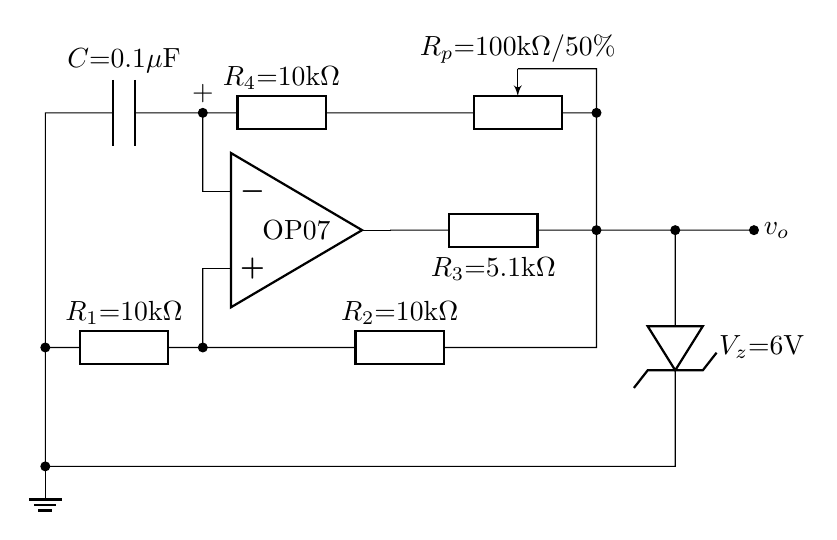
\begin{tikzpicture}[x = 2cm, y = 2cm]%方波
	\draw
	(0,0) node[op amp](AMP){} node[]{OP07};
	\draw
	let \p1 = (AMP.+), \p2 = (AMP.-), \p3 = (AMP.out) in
	(AMP.-) -- ++(0,0.5) node[circ](A){} node[anchor = south]{+} to [R = $R_4{=}10\text{k}\Omega$] ++(1,0) -- ++(0.5,0) to [pR, l^= $R_p{=}100\text{k}\Omega / 50\%$, n = pR] ++(1,0) -- ($(\x2, 0) + (2.5, 0)$) node[circ](B){} to [R = $R_3{=}5.1\text{k}\Omega$] (AMP.out)
	(AMP.+) -- ++(0,-0.5) node[circ](C){} to [R = $R_2{=}10\text{k}\Omega$] ($(\x2, \y1) + (2.5, -0.5)$) -- ($(\x2, 0) + (2.5, 0)$) -- ++(0.5,0) node[circ](O){} to [zzDo, l=$V_z{=}6\text{V}$] ++(0,-1.5) -- ($(\x1, 0) + (-1, -1.5)$) node[circ]{} node[ground]{} -- ($(\x1, \y1) + (-1, -0.5)$) node[circ](D){} to [R = $R_1{=}10\text{k}\Omega$] ++(1,0)
	(pR.wiper) -| ($(\x2, \y2) + (2.5, 0.5)$) node[circ]{}
	(D) -- ($(\x2, \y2) + (-1, 0.5)$) to [C = $C{=}0.1\mu\text{F}$] ++(1,0)
	($(\x2, 0) + (3, 0)$) to [short, -*] ++(0.5,0) node[anchor = west]{$v_o$};
\end{tikzpicture}
\caption{方波发生器电路图}\label{fig1}
\end{figure}
设电路通电瞬时,电容上的电压为零,电路输出为V$_z$,这时运放正向输入端电压为
\begin{equation}
V_{P1} = \cfrac{R_1}{R_1+R_2}V_z = FV_z\label{eq1}
\end{equation}
运放输出电流经$R_3$、$R_P$、$R_4$向电容C充电。运放反向输入端$V_N$随时间延续电压升高,当$V_N$=$V_{P1}$时,电路输出翻转,$V_o$由V$_z$变为-V$_z$,$V_P$由$V_{P1}$=FV$_z$变为$V_{P2}$=-FV$_z$。这时由“地”向电容反向充电,$V_N$随时间延续电压下降,当$V_N$=$V_{P2}$时,电路输出翻转,$V_o$由-V$_z$变为V$_z$,$V_P$由$V_{P2}$=-FV$_z$变为$V_{P1}$=FV$_z$。周而复始,电路输出方波。在稳态,输出为V$_z$的时间可用以下方法推导。在起始时刻,电容上的电压为$V_C$(0)=-FV$_z$,电容充电的终了电压为V$_z$,这里“电容充电的终了电压”指“若输出电压$V_o$不翻转,电容充电的终了电压”,所以电容上的电压为
\begin{equation}
V_c(t) = V_z + (-FV_z - V_z)e^{-\frac{t}{RC}}\label{eq2}
\end{equation}
其中,R=$R_P$+$R_4$。当电容上的电压达到FV$_z$时,电路翻转,记电容充电的时间为$\tau$,则
\begin{eqnarray*}
FV_z &=& V_z + (-FV_z - V_z)e^{-\frac{t}{RC}} \\
\tau &=& R\text{C}\text{ln}\cfrac{1+F}{1-F}
\end{eqnarray*}
输出方波的周期为2$\tau$。所以,输出方波的周期为
\begin{equation}
T = 2(R_P + R_4)\text{C}\text{ln}\left(1+\cfrac{2R_1}{R_2}\right)\label{eq3}
\end{equation}
所以,在实验中通过改变$R_P$就可以该变电路输出方波的周期。

通常,由于运放最大输出电流小于稳压二极管的最大稳压电流$I_{zmax}$,为使运放能正常工作,必须有限流电阻$R_3$。若电路不起振,可适当减小$R_3$的阻值。观察$V_C$、$V_o$的波形,并与理论分析的结果相比较。

\textbf{实验内容:}
\begin{enumerate}
\item 分别测量$R_4$+$R_P$=20k$\Omega$、40 k$\Omega$、60 k$\Omega$、80k$\Omega$、100k$\Omega$时电路输出波形的峰峰值和周期,记录波形,并与理论分析的结果相比较。
\end{enumerate}
\subsection{占空比可调的矩形波发生器}
电路如图(\ref{fig3})。与方波发生器相比,给C正向充电和反向充电使用了不同的路径,从而使得高电平持续时间和低电平持续时间不同。
\begin{figure}[!h]
\centering
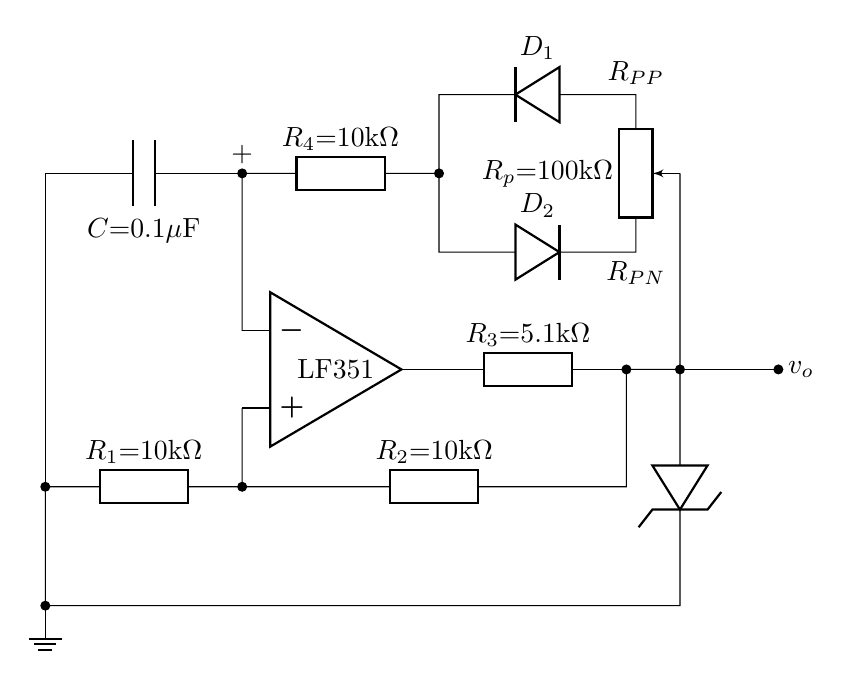
\begin{tikzpicture}[x = 2.5cm, y = 2cm]%可调方波
	\draw
	(0,0) node[op amp](AMP){} node[]{LF351};
	\draw
	let \p1 = (AMP.+), \p2 = (AMP.-), \p3 = (AMP.out) in
	(AMP.-) -- ++(0,1) node[circ](A){} node[anchor = south]{+} to [R = $R_4{=}10\text{k}\Omega$, -*] ++(1,0) -- ++(0,-0.5) to [Do, l^= $D_2$] ++(1,0) node[anchor = north]{$R_{PN}$} to [pR, n = pR, mirror, l^=$R_p{=}100\text{k}\Omega$] ++(0,1) node[anchor = south]{$R_{PP}$} to [Do, l_=$D_1$] ++(-1,0) -- ++(0,-0.5);
	\draw
	let \p1 = (AMP.+), \p2 = (AMP.-), \p3 = (AMP.out), \p4 = (pR.wiper) in
	(AMP.+) -- ++(0,-0.5) node[circ](B){} to [R = $R_2{=}10\text{k}\Omega$] ($(\x3, \y1) + (1, -0.5)$) -- ($(\x3, \y3) + (1, 0)$) to [short, *-] ($(\x4, 0)$) node[circ](O){} -- (pR.wiper)
	(O) to [zzDo] ++(0,-1.5) -- ($(\x1, \y3) + (-1, -1.5)$) node[ground]{} to [short, *-*] ($(\x1, \y1) + (-1, -0.5)$) to [R = $R_1{=}10\text{k}\Omega$] ++(1,0);
	\draw
	let \p1 = (AMP.+), \p2 = (AMP.-), \p3 = (AMP.out), \p4 = (pR.wiper) in
	(O) to [short, -*] ++(0.5,0) node[anchor = west]{$v_o$};
	\draw
	let \p1 = (AMP.+), \p2 = (AMP.-), \p3 = (AMP.out), \p4 = (pR.wiper) in
	(A) to [C = $C{=}0.1\mu\text{F}$] ++(-1,0) -- ($(\x1, \y1) + (-1, -0.5)$);
	\draw
	let \p1 = (AMP.+), \p2 = (AMP.-), \p3 = (AMP.out), \p4 = (pR.wiper) in
	(AMP.out) to [R = $R_3{=}5.1\text{k}\Omega$] ++(1,0);
\end{tikzpicture}
\caption{占空比可调的矩形波发生器电路图}\label{fig3}
\end{figure}
当输出为高电平V$_z$ 时,运放输出的电流经$R_{PP}$、$D_1$、$R_4$向电容充电,类同于对方波发生器的分析,忽略二极管的开启电压,容易得到输出高电平持续的时间
\begin{equation}
\tau_1 = (R_{PP}+R_4)\text{C}\text{ln}\left(1+\cfrac{2R_1}{R_2}\right)\label{eq4}
\end{equation}
类似地可以求得输出低电平持续的时间
\begin{equation}
\tau_2 = (R_{PN}+R_4)\text{C}\text{ln}\left(1+\cfrac{2R_1}{R_2}\right)\label{eq5}
\end{equation}
输出的周期为
\begin{equation}
T = \tau_1+\tau_2 = (R_P+2R_4)\text{C}\text{ln}\left(1+\cfrac{2R_1}{R_2}\right)\label{eq6}
\end{equation}
占空比
\begin{equation}
\eta = \cfrac{\tau_1}{\tau_2} = \cfrac{R_{PP}+R_4}{R_{PN}+R_4}\label{eq7}
\end{equation}
\textbf{实验内容:}
\begin{enumerate}
\item 调整$R_P$,分别测量$R_4$+$R_{PP}$=20k$\Omega$、40 k$\Omega$、60 k$\Omega$、80k$\Omega$、100k$\Omega$时电路输出波形的幅值、周期和占空比,并与理论分析的结果相比较。
\item 将占空比调为1,测量二极管导通时的电压降,计及二极管导通时的电压降,推导图(\ref{fig3}) 所示电路周期,并与测量结果相比较。
\end{enumerate}
\subsection{三角波发生器}
电路如图(\ref{fig4})。它由一个过零比较器和一个积分器组成。其工作原理可试述如下。
\begin{figure}[!h]
\centering
\begin{tikzpicture}[x = 1.8cm, y = 2cm]%三角
	\draw
	(0,0) node[op amp](AMP1){} node[]{\footnotesize AR1,OP07}
	(5,0) node[op amp](AMP2){} node[]{\footnotesize AR2,OP07};
	\draw
	let \p1 = (AMP1.+), \p2 = (AMP1.-), \p3 = (AMP1.out), \p4 = (AMP2.+), \p5 = (AMP2.-), \p6 = (AMP2.out) in
	(AMP.-) -- ++(-1,0) node[ground]{}
	(AMP.+) -- ++(-0.5, 0) -- ++(0,-1) node[circ](N1){} to [R = $R_1{=}10\text{k}\Omega$] ++(3,0) node[circ](N2){} -- ($(\x1,\y3)+(2.5,0)$) node[anchor = west](){$v_{o1}$} node[](VO1){} to [R = $R_2{=}5.1\text{k}\Omega$] (AMP1.out);
	\draw
	let \p1 = (AMP1.+), \p2 = (AMP1.-), \p3 = (AMP1.out), \p4 = (AMP2.+), \p5 = (AMP2.-), \p6 = (AMP2.out) in	
	(N1) to [pR = $R_p{=}22\text{k}\Omega/50\%$, n = pR, mirror] ++(0,-2) -| (AMP2.out)
	(pR.wiper) |- (N1);
	\draw
	let \p1 = (AMP1.+), \p2 = (AMP1.-), \p3 = (AMP1.out), \p4 = (AMP2.+), \p5 = (AMP2.-), \p6 = (AMP2.out) in
	(N2) to [zzDo, l= $V_z{=}6\text{V}$] ++(0,-1) node[ground](GND){};
	\draw
	let \p1 = (AMP1.+), \p2 = (AMP1.-), \p3 = (AMP1.out), \p4 = (AMP2.+), \p5 = (AMP2.-), \p6 = (AMP2.out), \p7 = (GND), \p8 = (VO1) in
	(GND) node[circ]{} -- ($(\x4,\y7)$) to [R = $R_4{=}10\text{k}\Omega$] (AMP2.+);
	\draw
	let \p1 = (AMP1.+), \p2 = (AMP1.-), \p3 = (AMP1.out), \p4 = (AMP2.+), \p5 = (AMP2.-), \p6 = (AMP2.out), \p7 = (GND), \p8 = (VO1) in
	(VO1) to [short, *-] ($(\x8,\y2)$) to [R=$R_3{=}10\text{k}\Omega$] (AMP2.-) node[circ]{} -- ++(0,1) to [C = $C{=}0.22\mu\text{F}$] ($(\x6,\y5)+(0,1)$) -- (AMP2.out) node[circ]{} -- ++(0.5,0) node[circ]{} node[anchor = west]{$v_o$};
\end{tikzpicture}
\caption{锯齿波发生器电路图}\label{fig4}
\end{figure}
设电路通电瞬时,t=0,电容上的电压为零,积分器输出$V_o$=0,过零比较器输出为$V_{o1}$=V$_z$,这时运放AR1正向输入端电压为
\begin{equation}
V_{P1} = \cfrac{R_P}{R_1+R_P}(V_z - V_o) = \cfrac{R_P}{R_1+R_P}V_z + \cfrac{R_1}{R_1+R_P}V_0 > 0\label{eq8}
\end{equation}
运放AR1输出保持为高电平。积分器输出线性地下降。当$V_{P1}$等于零时刻$\tau$,过零比较器翻转,$V_{o1}$=$-$V$_z$,记此时刻的积分器输出电压值为$V_{oN}$,
\begin{equation*}
\cfrac{R_P}{R_1+R_P}V_z = -\cfrac{R_1}{R_1+R_P}V_{oN}
\end{equation*}
由上式可解得
\begin{equation}
V_{oN} = -\cfrac{R_P}{R_1}V_z\label{eq9}
\end{equation}
不难得到三角波的周期4$\tau$。
\begin{equation}
V_{oN} = -\cfrac{1}{R_3C}\int_{0}^{\tau}V_z\text{d}t = -\cfrac{V_z}{R_3C}\tau\label{eq10}
\end{equation}
将(\ref{eq9})式代入(\ref{eq10})式可得到三角波的周期T
\begin{equation}
T = \cfrac{4R_3R_PC}{R_1}\label{eq11}
\end{equation}
还可以得到三角波的幅值为
\begin{equation}
V_{om} = \cfrac{R_P}{R_1}V_z\label{eq12}
\end{equation}
\textbf{实验内容:}
\begin{enumerate}
\item 取$R_P$=10k$\Omega$,观察电路输出波形$V_o$、$V_{o1}$,测量输出波形的周期和幅值。
\item 要求改变三角波的周期,可调整哪个元件,实验并测量记录之。
\end{enumerate}
\subsection{锯齿波发生器}
电路如图(\ref{fig6})。
\begin{figure}[!h]
\centering
\begin{tikzpicture}[x = 1.7cm, y = 2cm]%锯齿
	\draw
	(0,0) node[op amp](AMP1){} node[]{\footnotesize AR1,OP07}
	(6.5,-1) node[op amp](AMP2){} node[]{\footnotesize AR2,OP07}
	(AMP1.up) -- ++(0,0.1) node[anchor = west]{$+$}
	(AMP1.down) -- ++(0,-0.1) node[anchor = west]{$-$}
	(AMP2.up) -- ++(0,0.1) node[anchor = west]{$+$}
	(AMP2.down) -- ++(0,-0.1) node[anchor = west]{$-$};
	\draw
	let \p1 = (AMP1.+), \p2 = (AMP1.-), \p3 = (AMP1.out), \p4 = (AMP2.+), \p5 = (AMP2.-), \p6 = (AMP2.out) in
	(AMP.-) -- ++(-1,0) node[ground]{}
	(AMP.+) -- ++(-0.5, 0) -- ++(0,-1) node[circ](N1){} to [R = $R_2{=}10\text{k}\Omega$] ++(3,0) node[circ](N2){} -- ($(\x1,\y3)+(2.5,0)$) node[anchor = south](){$v_{o1}$} node[](VO1){} to [R = $R_3{=}5.1\text{k}\Omega$] (AMP1.out);
	\draw
	let \p1 = (AMP1.+), \p2 = (AMP1.-), \p3 = (AMP1.out), \p4 = (AMP2.+), \p5 = (AMP2.-), \p6 = (AMP2.out) in	
	(N1) to [short] ++(0,-2) to [R = $R_1{=}10\text{k}\Omega$] ($(\x6,\y1)+(0,-3)$) -- (AMP2.out);
	\draw
	let \p1 = (AMP1.+), \p2 = (AMP1.-), \p3 = (AMP1.out), \p4 = (AMP2.+), \p5 = (AMP2.-), \p6 = (AMP2.out) in
	(N2) to [zzDo, l= $V_z{=}6\text{V}$] ++(0,-1) node[ground](GND){};
	\draw
	let \p1 = (AMP1.+), \p2 = (AMP1.-), \p3 = (AMP1.out), \p4 = (AMP2.+), \p5 = (AMP2.-), \p6 = (AMP2.out), \p7 = (N2) in
	(N2) to [D-, l= $D_2{,}\text{1N4148}$] ++(1.5,0) node[anchor = north]{$R_{PN}$} to [pR, l_= $R_p{=}100\text{k}\Omega/90\%$, mirror, n = pR] ($(\x7,\y3)+(1.5,0)$) node[anchor = south]{$R_{PP}$} to [D-, l_= $D_2{,}\text{1N4148}$, -*] ++(-1.5,0);
	\draw
	let \p1 = (AMP1.+), \p2 = (AMP1.-), \p3 = (AMP1.out), \p4 = (AMP2.+), \p5 = (AMP2.-), \p6 = (AMP2.out), \p7 = (pR.wiper) in
	(pR.wiper) -- ($(\x7,\y3)$) to [R = $R_4{=}10\text{k}\Omega$] ++(2,0) node[circ](N3){} to [C = $C{=}0.22\mu\text{F}$] ($(\x6,\y3)$) node[anchor = south]{+} |- (AMP2.out)
	(N3) |- (AMP2.-);
	\draw
	let \p1 = (N3), \p2 = (GND), \p3 = (AMP2.+) in
	(GND) to [short, *-] ($(\x1,\y2)$) to [R = $R_5{=}10\text{k}\Omega$] ($(\x1,\y3)$) -- (AMP2.+);
	\draw
	(AMP2.out) node[circ]{} -- ++(0.5,0) node[circ]{} node[anchor = south]{$v_o$};
\end{tikzpicture}
\caption{三角波发生器电路图}\label{fig6}
\end{figure}
与图(\ref{fig4})三角波发生器相比,不同之处是:给C正向充电和反向充电使用了不同的路径,从而使得输出$V_{o1}$上升持续时间和下降持续时间不同。电容反向充电电流经过C、$R_4$、$R_{PN}$、$D_2$,类似于对三角波周期的推导,忽略二极管的开启电压,容易得到锯齿波的下降时间为
\begin{equation}
\tau_2 = \cfrac{2(R_{PN}+R_4)R_1C}{R_2}\label{eq13}
\end{equation}
电容正向充电电流经过C、$R_4$、$R_{PP}$、$D_1$,忽略二极管的开启电压,容易得到锯齿波的上升时间为
\begin{equation}
\tau_1 = cfrac{2(R_{PP}+R_4)R_1C}{R_2}\label{eq14}
\end{equation}
锯齿波的周期为
\begin{equation}
T = \tau_1+\tau_2 = \cfrac{2(R_P+2R_4)R_1C}{R_2}\label{eq15}
\end{equation}
类似于对三角波幅值的推导,容易得到锯齿波的幅值为
\begin{equation}
V_{om} = \cfrac{R_1}{R_2}V_z\label{eq16}
\end{equation}
\textbf{实验内容:}
\begin{enumerate}
\item 观察电路的输出波形,测量输出波形的上升时间$\tau$1 和下降时间$\tau$2。
\item 取$R_{PP}$分别为10k$\Omega$、30k$\Omega$、50k$\Omega$、70k$\Omega$、90k$\Omega$,测量输出波形$V_o$的$\tau$1 、$\tau$2的变化,并与理论估算值比较.
\item 将$D_1$、$D_2$反接输出波形$V_o$将发生什么变化?
\item 要求改变输出波形的周期,宜改变哪一个元件的元件值?测量记录之。
\end{enumerate}
\subsection{正弦波发生器}
电路如图(\ref{fig7})。
\begin{figure}[!h]
\centering
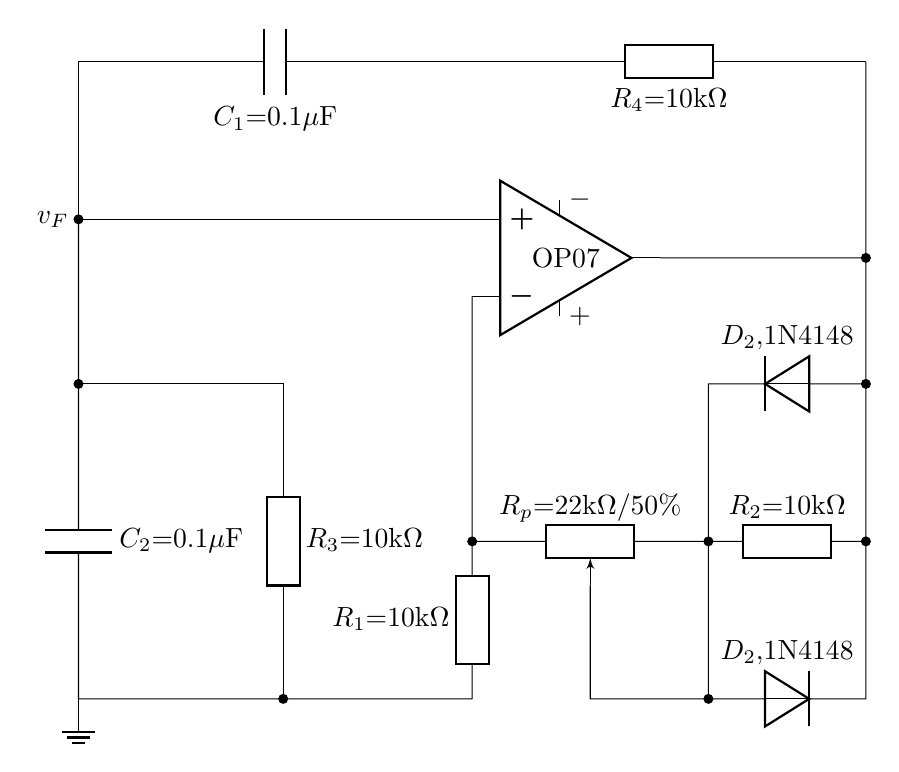
\begin{tikzpicture}[x = 2cm, y = 2cm]%正弦
	\draw
	(0,0) node[op amp, yscale = -1](AMP){} node[]{OP07}
	(AMP.down) -- ++(0,0.1) node[anchor = west]{$-$}
	(AMP.up) -- ++(0,-0.1) node[anchor = west]{$+$};
	\draw
	let \p1 = (AMP.+), \p2 = (AMP.-), \p3 = (AMP.out) in
	(AMP.+) -- ++(-2.5,0) node[circ](VF){} node[anchor = east]{$v_F$} -- ++(0,1) to [C, l_= $C_1{=}0.1\mu\text{F}$] ($(\x1,\y1)+(0,1)$) to [R, l_= $R_4{=}10\text{k}\Omega$] ($(\x1,\y1)+(2.5,1)$);
	\draw
	let \p1 = (AMP.+), \p2 = (AMP.-), \p3 = (AMP.out) in
	($(\x1,\y1)+(2.5,1)$)-- ($(\x1,\y3)+(2.5,0)$) node[circ](OUT){} -- ++(0,-0.8) node[circ](N1){} to [D-, l_=$D_2{,}\text{1N4148}$] ++(-1,0) -- ++(0,-2) node[circ](N2){} to [D-, l=$D_2{,}\text{1N4148}$] ++(1,0) -- ++(0,1) node[circ](N3){} to [R, l_= $R_2{=}10\text{k}\Omega$, -*] ++(-1,0) to [pR, l_=$R_p{=}22\text{k}\Omega/50\%$, n = pR] ($(\x2,\y3)+(0,-1.8)$) node[circ](N4){} to [R, l_= $R_1{=}10\text{k}\Omega$] ++(0,-1) -- ++(-1.2,0) node[circ](N5){} -- ++(-1.3,0) node[ground]{} to [C, l_= $C_2{=}0.1\mu\text{F}$] ++(0,2) node[circ](N6){} -- (VF)
	(OUT) -- (AMP.out)
	(N3) -- (N1)
	(pR.wiper) |- (N2)
	(N4) -- (AMP.-);
	\draw
	(N5) to [R, l_= $R_3{=}10\text{k}\Omega$] ++(0,2) -- (N6);
\end{tikzpicture}
\caption{正弦波发生器电路图}\label{fig7}
\end{figure}
该电路有一条正反馈支路,$R_4$、$C_1$、$R_3$、$C_2$。反馈系数为
\begin{equation}
F = \cfrac{V_F}{V_o} = \cfrac{R_3C_1s}{R_3R_4C_1C_2s^2+(R_3C_2+R_4C_1+R_3C_1)s+1}\label{eq17}
\end{equation}
若取$R_3$=$R_4$=R,$C_1$=$C_2$=C,则对于$\omega_o$=$\frac{1}{RC}$,有F=$\frac{1}{3}$。还有一条负反馈支路,$D_1$、$D_2$、$R_2$、$R_P$、$R_1$。该支路与运放组成了同相输入放大器,放大倍数为
\begin{equation}
A_{VF} = 1+\cfrac{R_P+R_{eq}}{R_1}\label{eq18}
\end{equation}
其中,$R_{eq}$为$D_1$、$D_2$、$R_2$的等效电阻。

振荡器起振的条件是:
幅值条件:|$\dot{A}_{VF}$F|$>$1; 
相位条件:$\sum\varphi = 2k\pi$, k=0,$\pm$1, $\pm$2$\dots$。
对于$\omega_o$正反馈支路的相移为0,所以只要$A_{VF}>$3,电路就能起振。

对于正弦波振荡器,起振后的平衡条件是:
幅值条件:|$\dot{A}_{VF}$F|=1; 
相位条件:$\sum\varphi = 2k\pi$, k=0,$\pm$1, $\pm$2$\dots$。
因此,电路一定要有自动调节的能力。在本电路中,在起振的瞬间,输出正弦波的幅值较小,其在电阻$R_2$上的分压V$_{R2}$小于二极管的开启电压$V_{Dth}$,二极管不起作用,$R_{eq}$=$R_2$,假设$R_P$=15k$\Omega$,由(\ref{eq18})式可知,这时同相放大器的放大倍数为3.5倍,大于3倍,输出电压波形的幅值不断增大。随着输出电压波形的幅值不断增大,当V$_{R2}$=$V_{Dth}$时,二极管导通,$R_{eq}$减小,最终平衡于$A_{VF}$=3,电路输出稳定的正弦波。

正弦波的幅值的估算。在稳态,负反馈支路的电流在$R_1$上的压降为输出电压的三分之一
\begin{equation*}
\cfrac{V_o - V_{Dth}}{R_P+R_1}R_1 = \frac13V_o
\end{equation*}
从中可解出输出正弦波的幅值
\begin{equation*}
V_o = \cfrac{3R_1}{2R_1 - R_P}V_{Dth}
\end{equation*}
由于二极管在一个周期内,在导通、截止之间不断变化,所以输出的“正弦波”的质量并不好,电路非线性造成的谐波失真较大。有多种实现从|$\dot{A}_{VF}$F|$>$1到|$\dot{A}_{VF}$F|=1的电路,有的电路可使输出正弦波的谐波失真较小。

\textbf{实验内容:}
\begin{enumerate}
\item 调整$R_P$,使电路起振,且使输出波形的幅值为5V,这时的$R_P$的阻值为多少?
\item 再把$R_P$调到最大,观察输出波形$V_o$。
\end{enumerate}

\newpage
\section{实验数据}

\subsection{方波发生器}%scope 12345
\begin{table}[!h]
\centering
\caption{方波发生器数据}
\label{data1}
\begin{tabular}{|c|c|c|c|c|}
\hline
$R_P$/k$\Omega$ & 峰峰值$V_{PP}$/V & 周期测量值T/ms & 周期理论值T/ms & 周期误差 \\ \hline
10.057          & 11.9          & 3.2803    & 4.407     & -25.56\%  \\ \hline
30.0218         & 12            & 5.401     & 8.794     & -38.58\%  \\ \hline
50.0151         & 12            & 7.274     & 13.187    & -44.83\%  \\ \hline
70.156          & 12            & 9.061     & 17.612    & -48.55\%  \\ \hline
90.06           & 11            & 10.784    & 21.985    & -50.94\%  \\ \hline
\end{tabular}
\end{table}
\begin{figure}[!h]
\centering
\subfloat[$R_P$=10.057k$\Omega$]{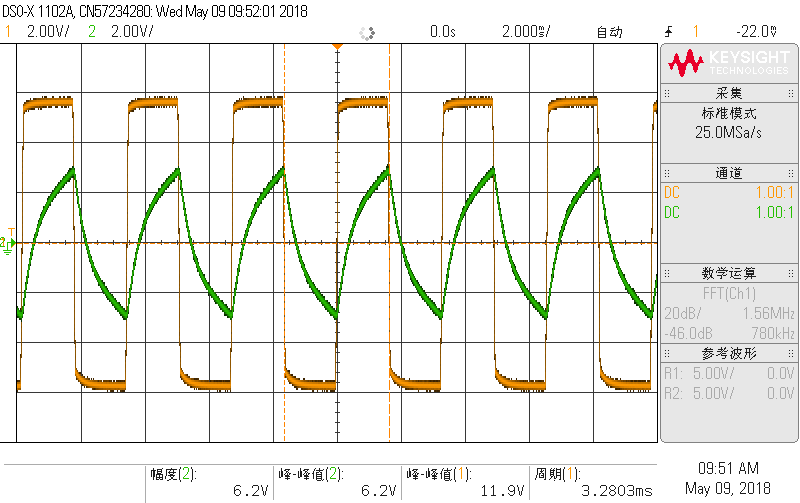
\includegraphics[width=0.45\textwidth]{fig/scope_1.png}}\qquad
\subfloat[$R_P$=30.0218k$\Omega$]{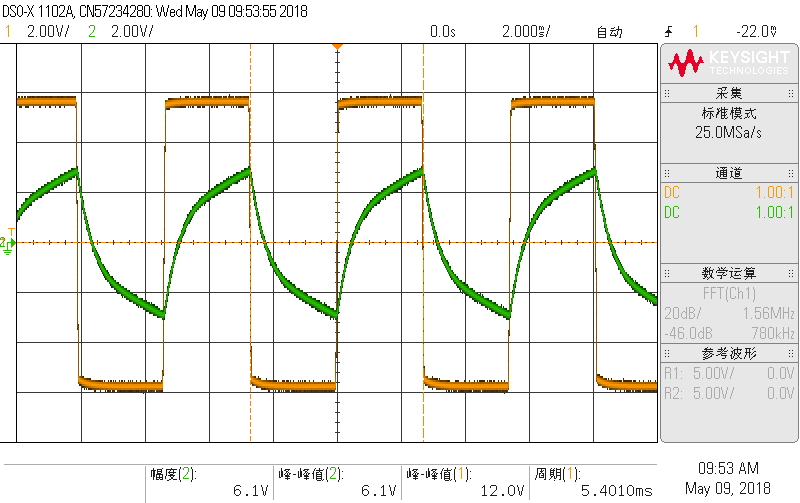
\includegraphics[width=0.45\textwidth]{fig/scope_2.png}}\qquad
\subfloat[$R_P$=50.0151k$\Omega$]{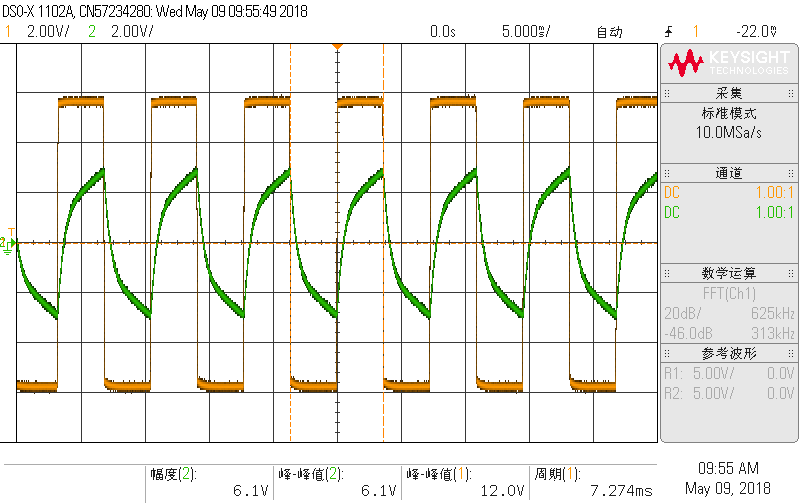
\includegraphics[width=0.45\textwidth]{fig/scope_3.png}}\qquad
\subfloat[$R_P$=70.156k$\Omega$]{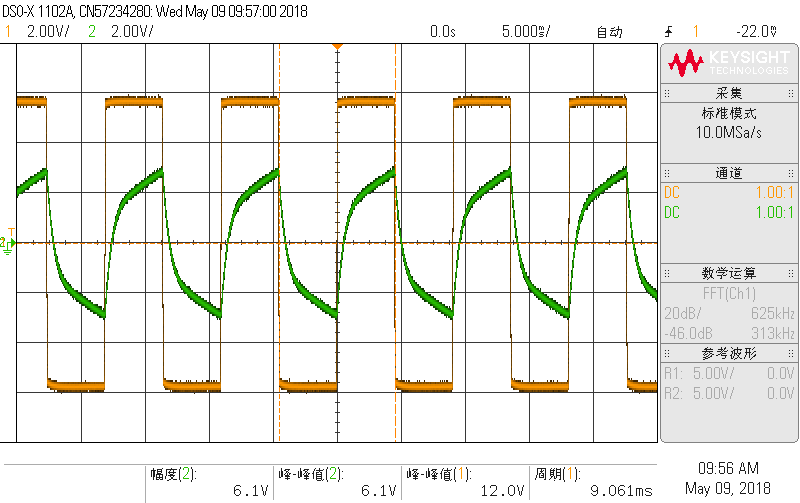
\includegraphics[width=0.45\textwidth]{fig/scope_4.png}}\qquad
\subfloat[$R_P$=90.060k$\Omega$]{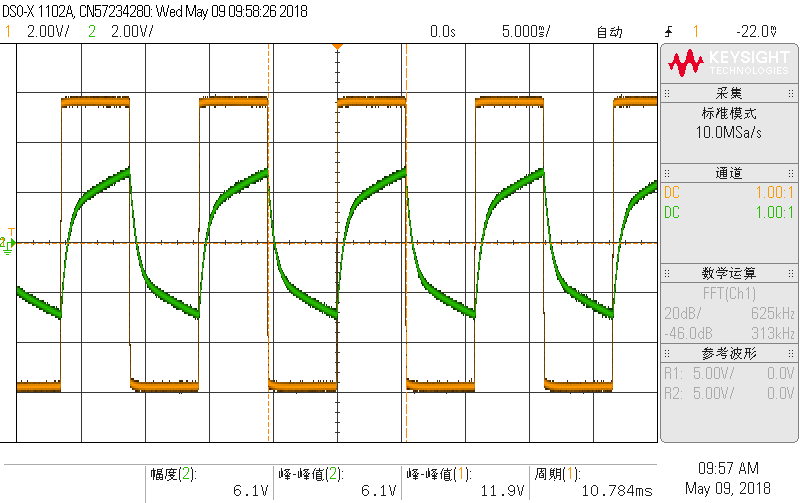
\includegraphics[width=0.45\textwidth]{fig/scope_5.png}}\\
\caption{方波发生器波形图}\label{datafig1}
\end{figure}

\newpage
\subsection{矩形波发生器}%scope 6789 10
\begin{table}[!h]
\centering
\caption{矩形波发生器数据}
\label{data2}
\begin{tabular}{|c|c|c|c|c|c|c|c|}
\hline
$R_P$/k$\Omega$ & $V_{PP}$/V & T(测量值)/ms & T(理论值)/ms & T误差    & $\eta$(测量值) & $\eta$(理论值) & $\eta$误差    \\ \hline
10.02           & 11.8          & 7.818     & 10.986    & -28.83670126 & 23.16\%      & 25.02\%      & -7.43\%  \\ \hline
30.042          & 11.9          & 8.026     & 10.986    & -26.94338249 & 37.36\%      & 41.7\%       & -10.40\% \\ \hline
50.077          & 12            & 8.071     & 10.986    & -26.53377025 & 50.15\%      & 58.4\%       & -14.12\% \\ \hline
70.026          & 12            & 8.022     & 10.986    & -26.97979246 & 62.96\%      & 75.02\%      & -16.07\% \\ \hline
90.053          & 11.9          & 7.801     & 10.986    & -28.99144366 & 77.34\%      & 91.71\%      & -15.66\% \\ \hline
\end{tabular}
\end{table}
\begin{figure}[!h]
\centering
\subfloat[$R_P$=10.020k$\Omega$]{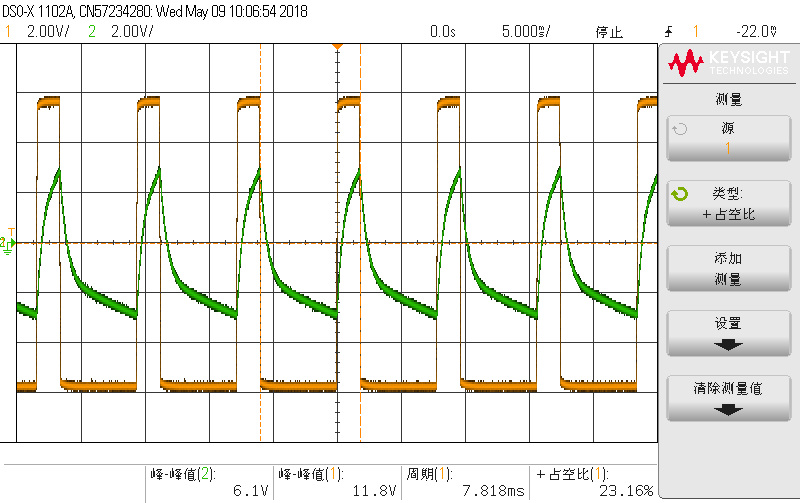
\includegraphics[width=0.45\textwidth]{fig/scope_6.png}}\qquad
\subfloat[$R_P$=30.042k$\Omega$]{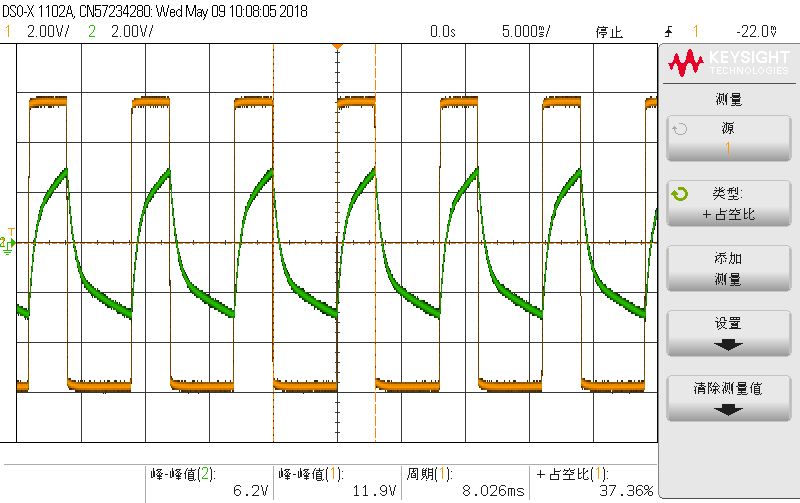
\includegraphics[width=0.45\textwidth]{fig/scope_7.png}}\qquad
\subfloat[$R_P$=50.077k$\Omega$]{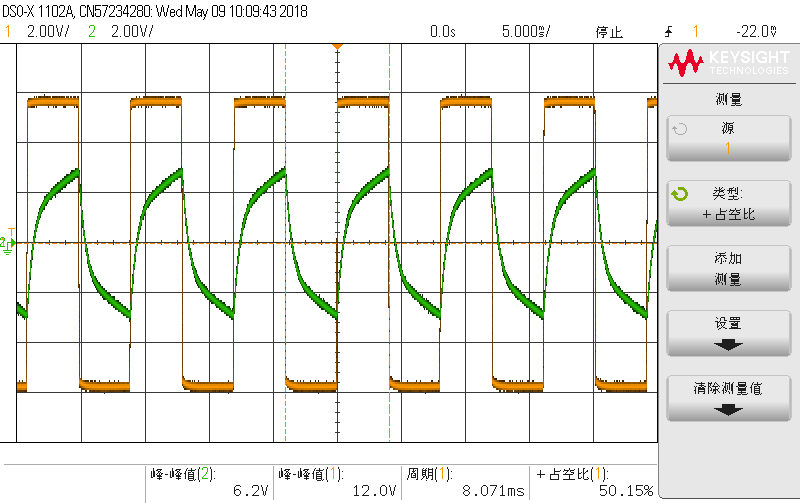
\includegraphics[width=0.45\textwidth]{fig/scope_8.png}}\qquad
\subfloat[$R_P$=70.026k$\Omega$]{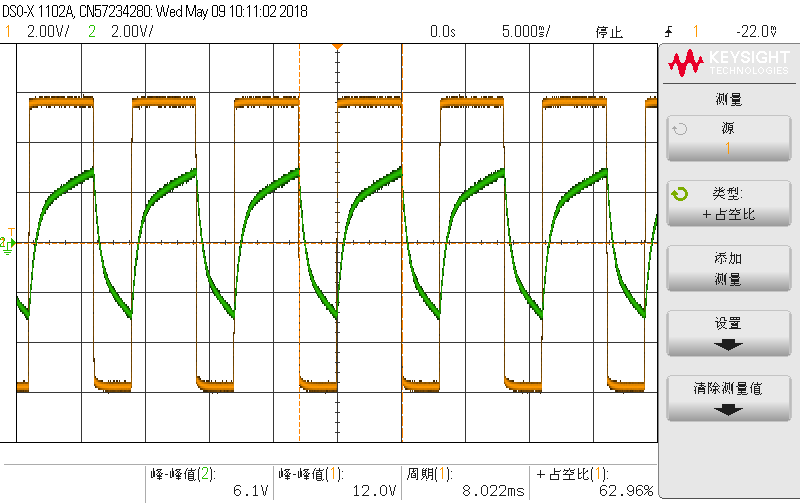
\includegraphics[width=0.45\textwidth]{fig/scope_9.png}}\qquad
\subfloat[$R_P$=90.053k$\Omega$]{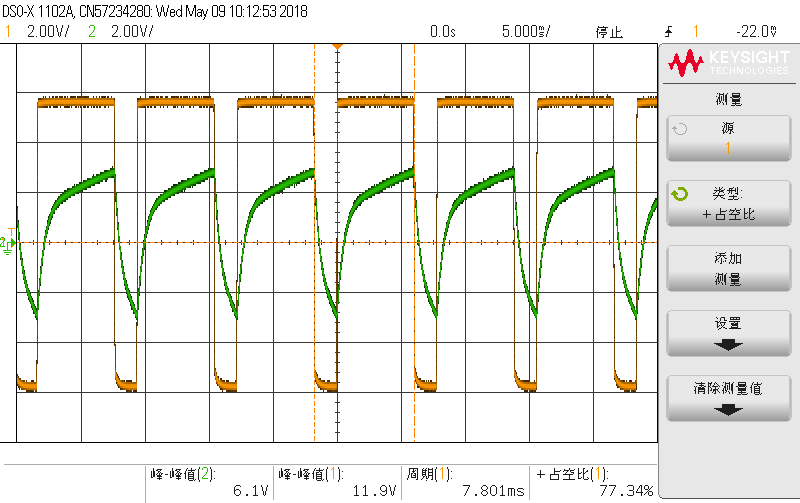
\includegraphics[width=0.45\textwidth]{fig/scope_10.png}}\\
\caption{矩形波发生器波形图}\label{datafig2}
\end{figure}

\newpage
\subsection{三角波发生器}%scope 11 12 13
\begin{table}[!h]
\centering
\caption{三角波发生器数据}
\label{data3}
\begin{tabular}{|c|c|c|c|c|}
\hline
$R_P$/k$\Omega$ & 峰峰值$V_{PP}$/V & 周期测量值T/ms & 周期理论值T/ms & 周期误差    \\ \hline
10.0466         & 11.1          & 9.498     & 8.841     & 7.43\%  \\ \hline
5.026           & 5.55          & 4.872     & 4.423     & 10.15\% \\ \hline
18.976          & 21.7          & 17.742    & 16.699    & 6.24\%  \\ \hline
\end{tabular}
\end{table}
\begin{figure}[!h]
\centering
\subfloat[$R_P$=10.0466k$\Omega$]{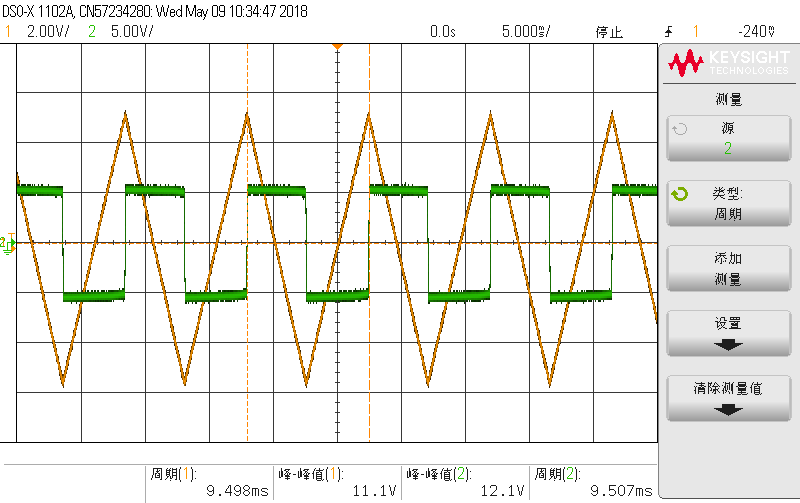
\includegraphics[width=0.45\textwidth]{fig/scope_11.png}}\qquad
\subfloat[$R_P$=5.0269k$\Omega$]{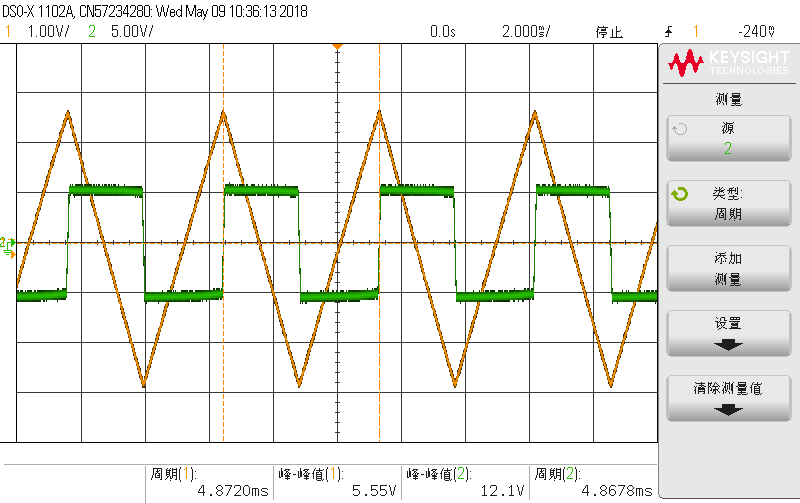
\includegraphics[width=0.45\textwidth]{fig/scope_12.png}}\qquad
\subfloat[$R_P$=18.976k$\Omega$]{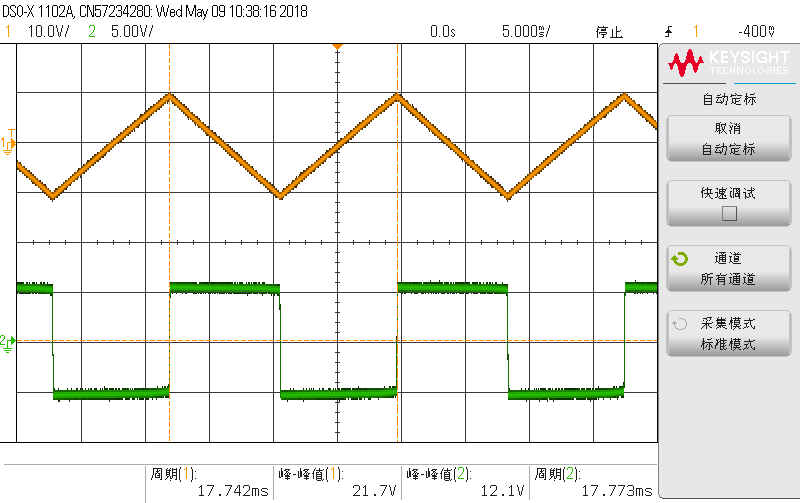
\includegraphics[width=0.45\textwidth]{fig/scope_13.png}}\\
\caption{三角波发生器波形图}\label{datafig3}
\end{figure}

\newpage
\subsection{锯齿波发生器}%scope 14 15
\begin{table}[!h]
\centering
\caption{锯齿波发生器数据:$D_1D_2$正接}
\label{data4:1}
\begin{tabular}{|c|c|c|c|c|c|c|c|}
\hline
$R_P$/k$\Omega$ & $V_{PP}$/V & T/ms  & 上升时间$\tau_1$ & 下降时间$\tau_2$ & 正脉宽$T_1$/ms & 负脉宽$T_2$/ms & 占空比$\eta$ \\ \hline
10.00538        & 12.1       & 62.33 & 8.62         & 41.22        & 51.71       & 10.71       & 82.84\%   \\ \hline
30.0187         & 11.9       & 62.85 & 16.74        & 32.64        & 41.74       & 21.18       & 66.34\%   \\ \hline
50.03           & 11.9       & 63.06 & 24.86        & 24.48        & 31.4        & 31.58       & 49.85\%   \\ \hline
70.0231         & 11.9       & 62.99 & 33.31        & 16.7         & 20.99       & 41.91       & 33.37\%   \\ \hline
90.0472         & 12.1       & 62.47 & 44.17        & 8.42         & 10.5        & 52.03       & 16.80\%   \\ \hline
\end{tabular}
\end{table}
\begin{table}[!h]
\centering
\caption{锯齿波发生器数据:$D_1D_2$反接}
\label{data4:2}
\begin{tabular}{|c|c|c|c|c|c|c|c|}
\hline
$R_P$/k$\Omega$ & $V_{PP}$/V & T/ms  & 上升时间$\tau_1$ & 下降时间$\tau_2$ & 正脉宽$T_1$/ms & 负脉宽$T_2$/ms & 占空比$\eta$ \\ \hline
10.0796         & 12.1       & 62.55 & 41.5         & 8.53         & 10.75       & 51.8        & 17.19\%   \\ \hline
30.044          & 11.9       & 62.91 & 33.19        & 16.94        & 21.22       & 41.68       & 33.73\%   \\ \hline
50.0191         & 11.9       & 62.94 & 24.98        & 25.22        & 31.62       & 31.38       & 50.19\%   \\ \hline
70.003          & 11.9       & 62.77 & 16.58        & 32.61        & 41.93       & 20.97       & 66.66\%   \\ \hline
90.0261         & 12.1       & 62.25 & 8.5          & 41.13        & 51.88       & 10.51       & 83.15\%   \\ \hline
\end{tabular}
\end{table}
\begin{figure}[!h]
\centering
\subfloat[$R_P$=10.00538k$\Omega$]{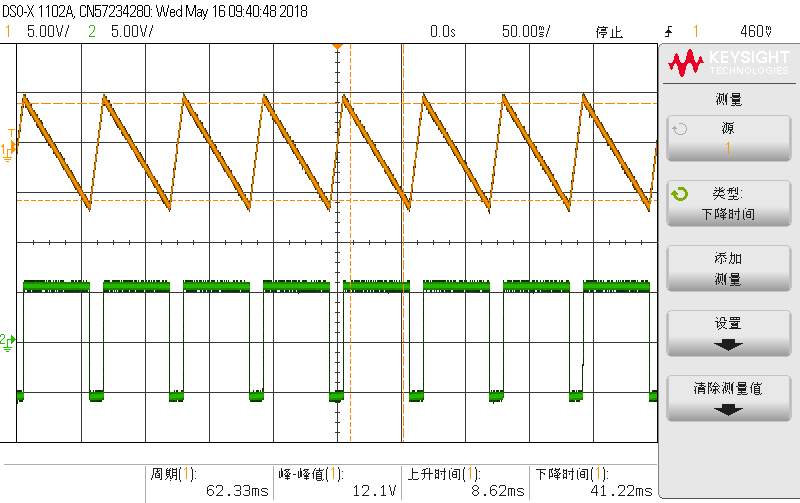
\includegraphics[width=0.45\textwidth]{fig/scope_14.png}}\qquad
\subfloat[$R_P$=30.0187k$\Omega$]{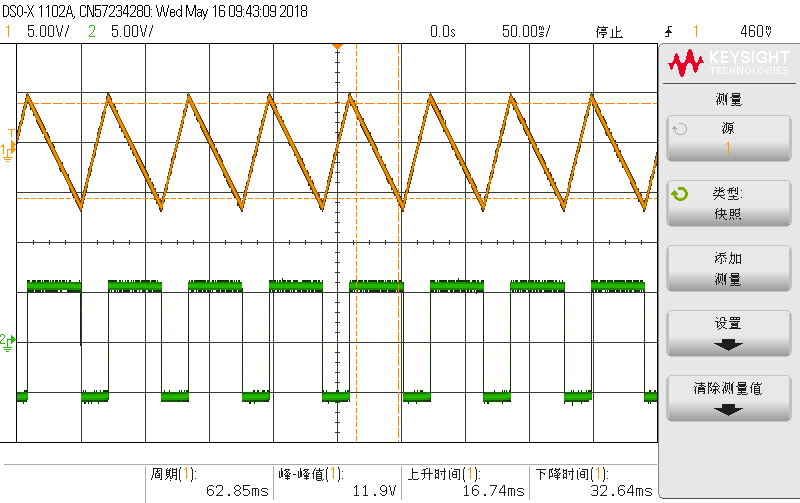
\includegraphics[width=0.45\textwidth]{fig/scope_15.png}}\\
\caption{锯齿波发生器波形图}\label{datafig4}
\end{figure}

\newpage
\subsection{正弦波发生器}%scope sin sin1
\begin{table}[!h]
\centering
\caption{正弦波发生器数据}
\label{data5}
\begin{tabular}{|c|c|}
\hline
$R_{PP}$/k$\Omega$ & $V_{PP}$/V \\ \hline
22.0573            & 5          \\ \hline
22.852             & 5.95       \\ \hline
\end{tabular}
\end{table}
\begin{figure}[!h]
\centering
\subfloat[$R_P$=22.0573k$\Omega$]{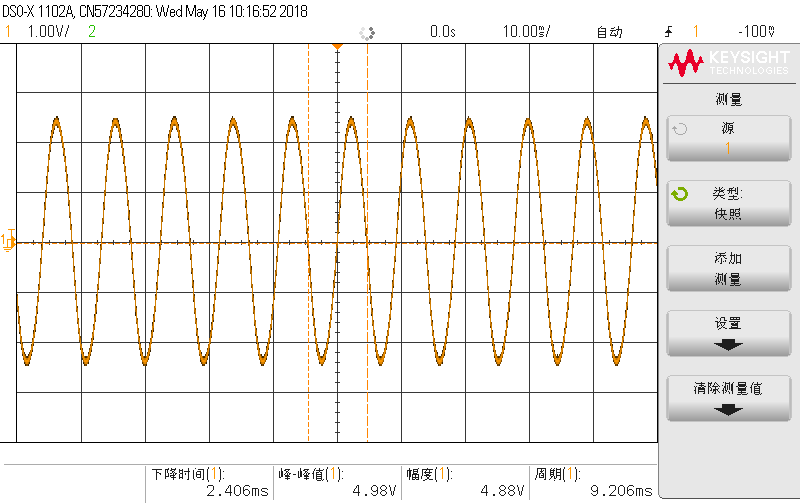
\includegraphics[width=0.45\textwidth]{fig/scope_sin.png}}\qquad
\subfloat[$R_P$=22.852k$\Omega$]{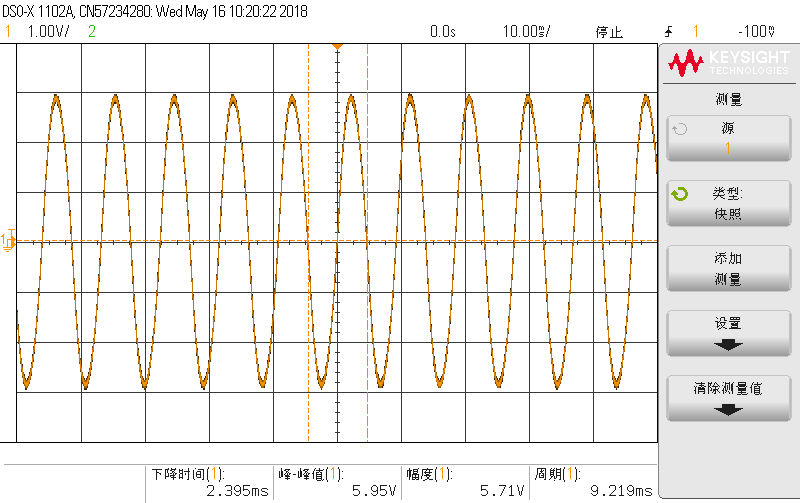
\includegraphics[width=0.45\textwidth]{fig/scope_sin1.png}}\\
\caption{正弦波发生器波形图}\label{datafig5}
\end{figure}

\section{实验讨论}
\iffalse
\begin{enumerate}
\item 锯齿波周期\\
从表((\ref{data4:1}))、(\ref{data4:2})中我们看到,锯齿波的周期并不等于测量得到的上升和下降时间之和。这是因为示波器测量上升下降时间时是取了变化范围的10\%和90\%处对应的时间值,因此相加不等于周期。
\item 正弦发生器输出截断\\
在实验过程中,其他同学将$R_P$调至最大时,输出信号会出现截断现象。但是我在实验过程中并没有观察到此现象。
\end{enumerate}
\fi

\section{思考题}
\subsection{图(\ref{fig1})中的$R_3$的阻值应如何选定?}
\subsection{图(\ref{fig1})所示电路中,电容C的容值应如何取?}
\subsection{在图(\ref{fig7})中,改变$R_P$时频率是否会随之变化?如电路已输出稳定的正弦波,改变$R_4$这时波形会发生什么变化?为什么?}
%\subsection{不改变图(\ref{fig7})中的正反馈电路,仅改变负反馈电路,使其输出正弦波的谐波失真较图(\ref{fig7})所示电路的小。请举出一个电路的例子,并说明原因。}

\nocite{jiaocai}
%--------bib------------------
\bibliography{ref.bib}
\end{document}